\keywords{Vera C. Rubin Observatory, LSST, Telemetry, Metrics, Time-series Databases}

\section{Introduction}

The Vera C. Rubin Observatory's Legacy Survey of Space and Time (LSST) represents the most ambitious and comprehensive optical astronomy survey ever planned. The LSST will survey the visible sky every few nights, generating a data stream of 20\,TB per night. The survey will produce a 500\,PB dataset over its ten-year lifetime, enabling a wide range of scientific investigations, from studying dark matter and energy to exploring the Solar System \cite{2019ApJ...873..111I}.

The LSST Data Management (DM) team is tasked with developing and maintaining the LSST Science Pipelines, which will process the data collected by the LSST. Additionally, the DM team oversees the performance of the LSST Science pipelines, ensuring that they meet the specifications outlined in the LSST Science Requirements Document (SRD). \cite{LPM-17}

Rubin Observatory also generates a large amount of telemetry data, which is used to monitor the observatory systems' health and troubleshoot issues during operations.

This paper describes Sasquatch, a service responsible for recording metrics and telemetry data from various subsystems at Rubin Observatory. The paper is organized as follows: Section~\ref{sec:tsd} provides an overview of the science performance metrics and telemetry data produced at Rubin Observatory and its representation as time series data. Section~\ref{sec:arch} describes the Sasquatch architecture. Section~\ref{sec:deploy} presents the Sasquatch deployments at Rubin Observatory. Section~\ref{sec:challenges} discusses the current challenges, and Section~\ref{sec:conc} concludes the paper.

\section{Time series data}
\label{sec:tsd}

Rubin Observatory will conduct several data processing campaigns during survey operations, such as "first look" analyses immediately after the images are captured by the LSST Camera, Prompt Processing handling approximately a thousand visits each night, and annual Data Release Processing campaigns. \cite{LSE-163} These campaigns will evaluate the quality of the data products through specific science performance metrics. \cite{2019ASPC..523..521B,2022SPIE12189E..0MG} These metrics have a timestamp and are measured across multiple dimensions (including instrument, detector, visit, filter, patch, and tract) understood by the data Butler \cite{2019ASPC..523..521B,2022SPIE12189E..0MG,2022SPIE12189E..11J}.

Telemetry is also timestamped data and measured across multiple dimensions. For example, the forces applied on the actuators of the LSST Primary/Tertiary mirror (M1M3) Active Optics System are measured at 50\,Hz and identified by the actuator number. Similarly, for the LSST Camera, telemetry data is measured for each amplifier, detector, and raft, among other dimensions.

Time series databases (TSDBs) are optimized for efficiently storing and querying timestamped data, making them ideal for metrics and telemetry data.

The following section describes the Sasquatch architecture, which leverages InfluxDB\footnote{\url{https://www.influxdata.com/time-series-database/}}, a popular TSDB.

\section{Sasquatch architecture}
\label{sec:arch}

Sasquatch\footnote{\url{https://sasquatch.lsst.io}} design provides data durability and high availability by combining InfluxDB and Apache Kafka\footnote{\url{https://kafka.apache.org}} deployed on the Kubernetes platform. \cite{SQR-029,SQR-068}

InfluxDB can handle high data throughput, making it suitable for writing and querying the high-frequency telemetry data produced by the Observatory Control System (OCS). In the current setup at USDF, data is replicated across two InfluxDB data nodes for redundancy, making it possible to write and query the database in case of a failure in one of the InfluxDB data nodes.

Apache Kafka is a distributed data streaming platform for high throughput and fault tolerance. Sasquatch uses the Strimzi operator\footnote{\url{https://strimzi.io}} to deploy Apache Kafka on Kubernetes. In Sasquatch, we replicate data across three Kafka brokers before writing to InfluxDB. When sending data to a Kafka topic representing a metric or a telemetry topic, Sasquatch requires an acknowledgment from at least two replicas for data durability.

Figure 1 shows the Sasquatch deployment at USDF, with InfluxDB, Kafka, and Kafka Connect being the main components. Kafka Connect runs MirrorMaker2, the connector responsible for mirroring the data from the Summit \cite{SQR-050}, and the InfluxDB Sink connectors responsible for consuming data from the Kafka brokers and writing to InfluxDB.

\begin{figure}[h]
    \centering
    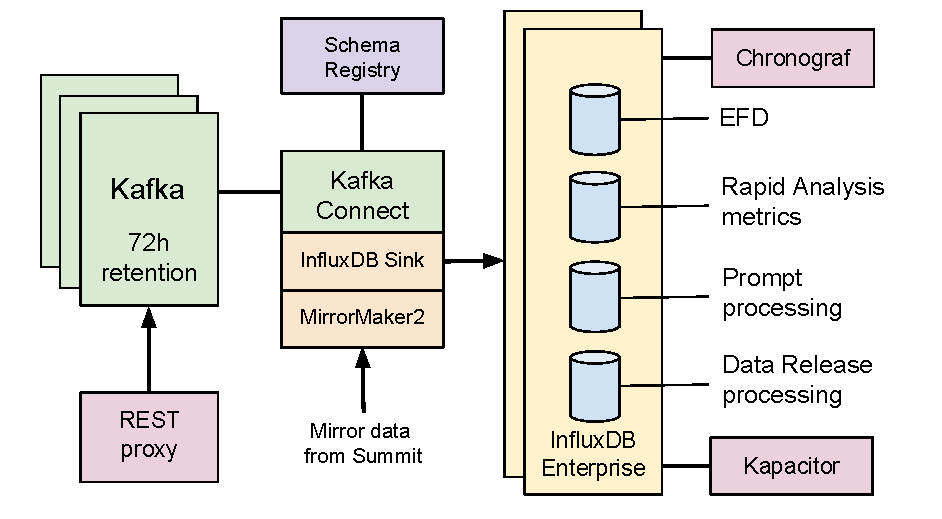
\includegraphics[width=0.8\textwidth]{figures/sasquatch-architecture.pdf}
    \caption{Sasquatch deployment at the US Data Facility.}
    \label{fig:system-architecture}

\end{figure}

Sasquatch manages multiple databases in InfluxDB to store data from various sources. For example, data produced by the OCS is routed to the Engineering and Facility Database (EFD) in InfluxDB. Similarly, metrics produced by the LSST Science Pipelines are routed to their corresponding databases, as illustrated in Figure 1. The routing mechanism is based on namespaces which are used to identify the data sources and the databases where the data should be stored.

\subsection{Sending data to Sasquatch}

Sasquatch uses Avro for the data serialization format and the Confluent Schema Registry (SR)\footnote{\url{https://docs.confluent.io/platform/current/schema-registry/}} to store the Avro schemas and ensure they can evolve safely, without breaking the Sasquatch consumers.

Applications connecting to Sasquatch can use native Kafka and SR clients to send data to Kafka. For example, the OCS Kafka producers\footnote{\url{https://ts-salkafka.lsst.io}} connect directly to Kafka and the SR to send data.

Alternatively, the REST Proxy\footnote{\url{https://docs.confluent.io/platform/current/kafka-rest/index.html}} provides a REST interface to Kafka. It makes connecting to Sasquatch easy, and it is a good solution when data rates are low. For example, the LSST Analysis Tools package uses the REST Proxy to send metrics from the LSST Pipelines outputs to Sasquatch.

\subsection{Data visualization, alerting, and analysis}

Enabling users to create dashboards and alerts is essential for monitoring and troubleshooting the observatory systems, especially during Rubin Observatory's current System Integration Testing and Commissioning (SITCOM) phase.

Sasquatch uses Chronograf for data visualization and Kapacitor for alert management. Dashboards and alert rules are defined using InfluxQL, a SQL-like query language with a rich set of functions specific to time series data analysis. Alert notifications are sent to particular channels on Slack to notify users about a metric excursion or the observatory system's health.

Sasquatch is also integrated with the Rubin Science Platform (RSP) \cite{DMTN-082, DMTN-212}. On the RSP at USDF, users can access data in real-time and historical data captured by Sasquatch. This integration enables users to analyze data in a JupyterLab environment with Python and leverage tools such as Times Square \cite{SQR-062} for publishing parameterized Jupyter Notebooks.

\section{Sasquatch deployments}
\label{sec:deploy}

Table 1 illustrates the various environments where we deploy Sasquatch, each with a different retention period, storage capacity, and target audience. Sasquatch deployments are managed by Phalanx\footnote{\url{https://phalanx.lsst.io}}, our Kubernetes-based internal developer platform for managing deployment configuration.

\begin{table}[ht]
    \small
    \centering
    \caption{Sasquatch environments at Rubin Observatory}
    \begin{tabular}{@{}llll@{}}
        \toprule
        \textbf{Environment} & \textbf{Retention Period} & \textbf{Current Capacity} & \textbf{Audience} \\
        \midrule
        Summit & 30 days & 5 TB & Staff at the Summit \\
        USDF & Project lifetime & 60 TB & Project at large \\
        IDF (Google Cloud Platorm) & 1 year & 30 TB & Project at large (online backup) \\
        Teststands (Tucson \& Base Facility) & 10 days & 1 TB & Developers \\
        \bottomrule
    \end{tabular}
\end{table}

At the Summit, we store data for 30 days, and the primary audience for this deployment is the observatory staff. At the USDF, we are required to keep the data for the project's lifetime and make it available to the project at large. We also deploy Sasquatch on the Google Cloud Platform, where we keep the last year of data as an online backup in case users cannot access Sasquatch at the USDF. Finally, we have independent test stand deployments in Tucson, US, and at the Base Facility in La Serena, Chile. At the test stands, we record simulated data, and the primary audience for these deployments is our developers.

\section{Challenges}
\label{sec:challenges}

During the Rubin Observatory construction phase, we have been collecting metrics to characterize the performance of the LSST Science Pipelines algorithms running on precursor datasets.  \cite{DMTN-091,2022SPIE12189E..0MG} At the observatory, we started collecting telemetry data in 2019 from the LSST Auxilary Telescope (AuxTel) runs and more recently during the SITCOM phase of the Main Telescope systems, notably M1M3 \cite{SITCOMTN-088}, Telescope Mount Assembly (TMA) \cite{SITCOMTN-121} and Secondary Mirror (M2) systems \cite{SITCOMTN-120}.

Even before the start of survey operations, we recorded 20\,TB of metrics and telemetry data in Sasquatch, with data rates peaking at 565\,GB/week \cite{SQR-085}. With the integration of the LSST Camera into the OCS, which is planned for this year, we expect the data rates to increase even further.

Table 2 shows the projected storage growth for the EFD database. From the data rates observed so far, we estimate that the size of the database will increase by 30\,TB yearly during survey operations. By the end of the 10-year survey, we expect around 1\,PB of data in Sasquatch.

\begin{table}[ht]
    \centering
    \caption{Projected storage size for the EFD at USDF by year considering a replication factor of two.}
    \begin{tabular}{@{}lllll@{}}
        \toprule
        \textbf{End of Year} & \textbf{EFD Size} & \textbf{RF} & \textbf{Total Storage} & \textbf{Main Drivers} \\
        \midrule
        2022 & 2 TB & 2 & - & AuxTel \\
        2023 & 15 TB + SM & 2 & 60 TB & M1M3, TMA, M2 + AuxTel \\
        2024 & 35 TB + SM & 2 & 100 TB & MainTel + AuxTel \\
        2025 & 65 TB + SM & 2 & 160 TB & Survey operations \\
        2035 & 0.3-0.5 PB + SM & 2 & 0.7-1 PB & Survey operations \\
        \bottomrule
    \end{tabular}
\end{table}

Managing a 1\,PB database on premises is challenging. We are responsible for maintaining the underlying hardware infrastructure, solving performance and scalability issues, ensuring data consistency between the Summit and USDF databases, performing database operations such as backups and restores, and providing data access tools to our users. In Sasquatch, we are working on several fronts to address these challenges.

We recently transitioned from InfluxDB OSS to an InfluxDB Enterprise cluster at USDF to improve database performance, scalability, and support. Currently, at the USDF, the InfluxDB Enterprise cluster has 2x8-core data nodes with 30\ TB of local SSD storage each and a replication factor (RF) of two for redundancy. To increase storage capacity, we can add more nodes to the cluster. We are constantly reviewing the projected storage size for the EFD at USDF (table 2) and expanding the cluster capacity as required. We are working closely with InfluxData support to understand the best practices for scaling InfluxDB and leverage the new features of the InfluxDB 3.0 clustered product, such as storage tiering and the fact that the latest version is Kubernetes native.

Ensuring consistency between the databases at the Summit and USDF is a critical task. To achieve this, we have adopted MirrorMaker2. This component at USDF is responsible for mirroring data from the Summit. It can automatically recover data from network outages shorter than the Kafka retention period, which is currently set to 72 hours. If data is present in Kafka but missing in InfluxDB at USDF, we can deploy repairer connectors to replay the missing data to InfluxDB. This process is currently manual and triggered by data consistency checks between the Summit and USDF databases. In the event that the data is no longer present in Kafka, data recovery can still be performed by restoring database backups from the Summit to USDF. We are actively working on automating the data recovery process to significantly reduce the time required to recover data and to minimize the impact on users.

To improve data access to users, we are working on tools to aggregate telemetry data \cite{SQR-058} and export the data to formats like Apache Parquet and VO TAP (Table Access Protocol)\cite{2019ivoa.spec.0927D} to leverage existing data access mechanisms in the RSP.

Finally, we must continuously adapt as Sasquatch and OCS software components evolve. At the Summit, the OCS is adopting Kafka for the middleware implementation \cite{2024SPIE13101.59Ftmp, TSTN-033}. That means the OCS will record commands, events, and telemetry data directly in Kafka. In principle, Sasquatch and the OCS could share the same Kafka cluster, simplifying their integration and avoiding the duplication of resources and data. However, this will also bring new challenges we must address in the Kafka configuration. While the OCS needs to ensure low latency for commands and events, Sasquatch must prioritize data durability for recording telemetry data. We are working with the OCS team to understand the requirements and constraints of the new Kafka deployment and adapt Sasquatch to the new environment.

\section{Conclusion}
\label{sec:conc}

This paper provides a comprehensive overview of Sasquatch. Over the years, Sasquatch's design has evolved significantly, providing high availability and data durability for metrics and telemetry data. Sasquatch combines InfluxDB Enterprise and Apache Kafka to efficiently store and query time series data. Sasquatch is deployed in multiple environments at Rubin Observatory, each with different retention periods, storage capacity, and target audience.

Sasquatch enables real-time access to data mirrored from the Summit and historical data at the USDF. Sasquatch also leverages tools such as Chronograf for data visualization and Kapacitor for alert management and is integrated with the RSP notebook aspect for data analysis with Python.

While we are still improving the Sasquatch deployment at the USDF and Summit environments, InfluxDB Enterprise and Apache Kafka offer a solid foundation for Sasquatch. Sasquatch is currently employed during Rubin Observatory's SITCOM phase and is an essential service as we transition into survey operations.

\vskip 0.4in
